\chapter{Thermal instability in homogeneous plasmas} \label{ch: thermal instability}

\graphicspath{{03-thermal_instability/figures/}}

\usespublishedwork{Most of this Chapter was published in ``Thermal instabilities: Fragmentation and field misalignment of filament fine structure'', 2020, \aanda, 636, A112 \citep{claes2020}. N. Claes performed the simulations, analysed the data and wrote the manuscript. R. Keppens and C. Xia contributed to the revision of the paper. Some parts of this Chapter were also published in ``Thermal stability of magnetohydrodynamic modes in homogeneous plasmas'', 2019, \aanda, 624, A96 \citep{claes2019}. N. Claes performed the simulations, analysed the data and wrote the manuscript; R. Keppens contributed to the revision of the paper.}

\section{Introduction}

\section{The physics of thermal instability}
As already mentioned in the previous Chapter, in non-adiabatic MHD the stability of the thermal (entropy) mode is strongly dependent on the heat-loss function $\HLF$, which in general depends on the usual thermodynamic quantities like density and temperature, and in some cases also on the magnetic field through the choice of heating function. In our formalism however, i.e. following Equation \eqref{eq: cooling_simple}, the heating term $\HLFheat$ is assumed to be constant such that $\HLF$ only depends on density and temperature. The latter dependence enters by means of the cooling curve $\HLFcool$, which are tabulated values resulting from detailed atomic and molecular calculations. Due to the nature of these tables they have a rather coarse spread of datapoints, spanning multiple orders of magnitude in temperature. We therefore perform a local second-order polynomial interpolation at high resolution, where ``local'' means between two original data points, in order to preserve all data from the original table.
Figure \ref{fig: coolingcurves} shows two of these tables along with their interpolated curves as a function of temperature: blue denotes the curve given in \citet{colgan2008} (hereafter referred to as ``\jccorona''). The sharp drop near $10^4$ K is due to the ionisation of hydrogen, which essentially sets radiative cooling for lower temperatures to zero. Red on the other hand denotes the one given by \citet{schure2009} (hereafter referred to as ``\spexdm'') and is extended to lower temperatures using \citet{dalgarno1972}. Dots represent the original table values, solid lines denote the interpolated cooling curves.

\begin{figure}[t]
  \centering
  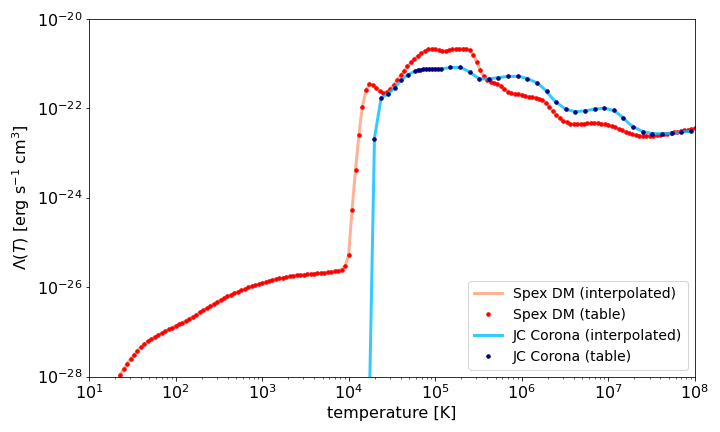
\includegraphics[width=\textwidth]{coolingcurves.png}
  \caption{
    Plots of two cooling curves $\HLFcool$ as a function of temperature. Red denotes the curve given by \citet{schure2009}, extended to low temperatures using \citet{dalgarno1972}. Blue denotes the curve given by \citet{colgan2008}. Dots represent values from the original tables, solid lines a local second-order polynomial approximation.
  }
  \label{fig: coolingcurves}
\end{figure}

Now, suppose a plasma that gains energy from an external source (constant heating in this case) and looses energy to its surroundings through optically thin radiative cooling processes (cooling), but is in full thermal equilibrium such that these two contributions cancel each other out (i.e. $\HLF_0 = 0$). This thermal equilibrium state will only be maintained if the plasma is stable with respect to small perturbations, such that any deviation from this state is counteracted and the plasma returns to its initial configuration.

Now assume that this plasma is at a certain uniform temperature at which $\dHLFT$ is negative, that is, the value of $\HLFcool$ increases when temperature decreases. This is the case at e.g. two million Kelvin (see Figure \ref{fig: coolingcurves}) for both cooling curves. If this plasma is perturbed such that the temperature decreases slightly, $\dHLFT < 0$ implies that the radiative losses will increase and the plasma looses even more energy, decreasing the temperature even further. This process will happen relatively slow at first, but after a while the plasma reaches a point of no return and a \emph{catastrophic cooling phase will kick in}: the small, initial perturbation that lowered the temperature grows and leads to \emph{thermal instability}. Nature's tendency is to keep pressure equilibrium, and according to the ideal gas law $p = \rho T$ the initial drop in temperature is accompanied by an increase in density in an (in this case futile) attempt to restore pressure balance. This has an adverse effect on the plasma as the heat-loss function $\HLF$ as defined here is linearly dependent on density, meaning that a density increase leads to more energy losses. This, combined with the continuing drop in temperature leads to a runaway cooling process: the plasma density keeps increasing while the temperature keeps decreasing, giving rise to high-density, low-temperature regions.
A density perturbation can also give rise to thermal instability in the same manner as before: an increase in density implies a decrease in temperature or vice-versa (pressure balance), hence a temperature disturbance and the possibility to trigger instability. The effect of $\dHLFT$ on the growth rate of thermal instability is in general much stronger than $\dHLFrho$, except in regions where the heat-loss function has a relatively flat temperature dependence. In those cases the disturbance in density may actually be the dominant mechanism to trigger instability instead of temperature, where the density changes lead to cooling/heating variations.

The above discussion treats the case in which energy losses increase for decreasing temperature, but the reverse (i.e. $\dHLFT > 0$) may also give rise to instability. Here a drop in temperature decreases the energy losses, such that the heating term becomes dominant and heats up the plasma. A similar runaway process starts, where plasma density now decreases in an attempt to restore pressure equilibrium, lowering radiative losses even further. Generally speaking this process can also be referred to as ``thermal instability'', this time driven by heating. However, both cases give rise to both high density and low density plasma regions, such that we will not distinguish between the two.

Plasmas that are thermally stable will eventually return to thermal equilibrium after small perturbations. Due to the strong link between stability and $\dHLFT$, this will mainly happen in regions where the temperature dependence is minor, that is, for flat regions in the cooling curves. One such region may be just below $10^5$ K on Figure \ref{fig: coolingcurves}: here a small perturbation will only lead to a minor change in heating and cooling, such that the system has enough time to counteract the imbalance before the runaway reaction occurs. This may not be sufficient for perturbations that are large enough however, due to the delicate interplay between the heating and cooling terms, such that they might still be able to trigger instability.

If thermal conduction is also present then this will \emph{always} have a stabilising effect on the thermal instability. Initial temperature perturbations will be smoothened out due to thermal conduction effects, and even if the runaway cooling process has already started it will try and continue to do so. Generally speaking this stabilising behaviour will lead to a reduction of the thermal instability growth rate, but actually \emph{preventing} instability will only occur in a few select cases. The high anisotropy of thermal conduction plays a major role in magnetised plasmas as the effect is several orders of magnitude stronger parallel to the magnetic field lines than across, allowing for strong temperature gradients across field lines (and hence large $\dHLFT$ values). This implies that the direction of the wave vector is important, since perturbations more parallel to the magnetic field will be strongly stabilised, while wave vectors (near) perpendicular to the field lines will undergo almost no stabilisation by thermal conduction.

All of the above, which assumes a plasma at uniform temperature and a constant heating term, is ideal to get an intuitive feeling what thermal instability is and how it originates. In reality however things are much more complicated: the plasma is certainly not uniform, and in general the heat-loss function will have a complicated dependency on other (thermodynamic) variables. This implies that the process of thermal instability is much more intricate in fully realistic plasmas with regard to (in)stability, but the general idea holds: an unstable thermal mode triggers a runaway radiative cooling reaction, which in turn leads to high-density, low-temperature condensations.


\section{Thermal instability and nonlinear fragmentation}
As explained in the previous Section thermal instability leads to condensations. What we are now interested in is the spontaneous emergence of fine structure in these high-density condensations and how this evolves under typical solar coronal conditions. As mentioned in the introductory part of this Chapter both solar prominences and coronal rain condensations most likely originate from thermal instabilities in the solar corona, and it is still not understood how non-linear instability evolution shapes the observed fine structure of prominences. Investigating this requires multi-dimensional, high-resolution simulations to resolve all emerging substructure in great detail. This is what we embark upon for the remainder of this Chapter. However, first we have to know under which conditions thermal instabilities can actually form. We already discussed the intricate dependence of thermal stability on the heat-loss function, which in turn implies that we have both stable and unstable regions. For this we need detailed knowledge of the growth rates of the various modes, which we can obtain by solving the eigenvalue problem. Once we have identified these regions of interest we can setup our numerical simulations.


\subsection{Eigenfunctions}
Before diving into the simulation aspect of this Chapter we first change the background orientation of the magnetic field vector and wave vector. We plan to perform numerical simulations of a given setup and the usual convention is to align the magnetic field itself with one of the coordinate axes -- just as we have been doing up to now. Here we will do the opposite: aligning the wave vector $\bk$ with the $x$-axis while the magnetic field $\bb_0$ will be aligned in the 3D coordinate system. The advantage of this is that we can use periodic boundary conditions on all sides of the domain in our numerical simulations. If we would have kept the general convention as-is then all waves would propagate at some arbitrary angle with respect to the coordinate axes, such that it would have been quite difficult to make use of periodic boundary conditions, even more so when imposing multiple waves on top of each other. We can therefore define $\bk$ and $\bb_0$ as follows
\begin{equation}
  \bk = (k_x, 0, 0), \qquad\qquad \bb_0 = \left(B_{0x}, B_{0y}, B_{0z}\right).
\end{equation}
Using this convention we can rewrite the system of linear MHD equations \eqref{eq: linearised_rho1_homo}-\eqref{eq: linearised_A1_homo} in terms of the unknown variables. This results in the eigenfunctions associated with a specific orientation of the wave vector $\bk$ with respect to the magnetic field $\bb_0$, given by
\begin{gather}
  \rho_1 = \frac{k_x \rho_0}{\omega}v_{1x}, \label{eq: rho1_eigenfunction}\\
  v_{1y} = \frac{B_{0x}B_{0y}k_x^2}{B_{0x}^2k_x^2 - \omega^2\rho_0}v_{1x}, \\
  v_{1z} = \frac{B_{0x}B_{0z}k_x^2}{B_{0x}^2k_x^2 - \omega^2\rho_0}v_{1x}, \\
  T_1 = -\frac{k_x \rho_0 \gmone \left(\icomplex\dHLFrho\rho_0 - T_0 \omega\right)}{
    \omega\left[
      \icomplex\gmone\left(\kappapara\kpara^2 + \kappaperp\kperp^2\right)
      + \icomplex\gmone \dHLFT \rho_0
      + \omega \rho_0
    \right]
  }v_{1x}, \\
  A_{1y} = \frac{\icomplex B_{0z}\omega \rho_0}{B_{0x}^2k_x^2 - \omega^2\rho_0}v_{1x}, \\
  A_{1z} = -\frac{\icomplex B_{0y}\omega \rho_0}{B_{0x}^2k_x^2 - \omega^2\rho_0}v_{1x}, \label{eq: A1Z_eigenfunction}
\end{gather}
where the eigenfunctions for the $x$-component of the vector potential $A_{1x} = 0$. All of the above eigenfunctions have a dependence on $v_{1x}$, such that this eigenfunction can be chosen arbitrarily. Similar results can be obtained when $\bk$ is aligned along a different coordinate axis or when shifting to 2D. The main advantage of having the actual eigenfunctions is that we can now consistently excite a specific MHD wave mode associated with a certain eigenvalue $\omega$ in numerical simulations. The eigenfrequency itself can be obtained by solving the eigenvalue problem just as we did before.

\subsection{Numerical setup}
To perform the simulations we make use of the parallelised Adaptive Mesh Refinement Versatile Advection Code MPI-AMRVAC \citep{keppens2012_amrvac,porth2014_amrvac,xia2018_amrvac} to numerically solve the full non-linear, non-adiabatic MHD equations on a two- or three-dimensional Cartesian mesh with multiple levels of adaptive mesh refinement (\gls{AMR}). The base resolution used in all simulations is $100^2$ and $100^3$ for the 2D and 3D results, respectively. Three (3D) and five (2D) levels of AMR are used with the trigger of refinement based on a density criterion, achieving a maximum effective resolution of $400^3$ and $1600^2$ near high-density regions in 3D and 2D, respectively. As indicated further, one ultra-high resolution run in 2D uses seven AMR levels for a $6400^2$ run to reveal more details. The length scale of the system is of the order of a few to 10 Mm depending on the simulation. In MPI-AMRVAC both the radiative cooling contribution and conduction effects are handled as additional source terms to the energy equation. \spexdm is used as a cooling curve, the heating term is taken to be constant over time and equal to the radiative losses at $t = 0$, implying that the radiative losses and heating contribution balance each other at $t = 0$ such that an initial state of thermal equilibrium is achieved. Thermal conduction is treated in full tensorial form, a detailed explanation on how the code handles conduction effects parallel and perpendicular to the magnetic field is provided in \citet{xia2018_amrvac}.

\subsubsection{Initial conditions}
We use periodic boundary conditions on all sides of the domain and start from a uniform thermal equilibrium state as described before. The wave vector $\bk$ is always equal to $2\pi$ divided by the domain length to ensure one single oscillation along one of the axes to satisfy the periodic boundary conditions on all sides (in other words, the wave ``fits'' nicely in the domain). The magnetic field orientation with respect to the coordinate axes is described by an angle $\theta$, measured from the $xy$-plane towards the $z$-axis, and by an angle $\delta$ measured in the $xy$-plane from the $x$-axis towards the $y$-axis. Using this description the background magnetic field $\bb_0$ can be written as
\begin{equation}
  \bb_0 = \left(B_0\cos\theta\cos\delta, B_0\cos\theta\sin\delta, B_0\sin\theta\right).
\end{equation}
In two dimensions the expression for $\bb_0$ becomes straightforward, as we only have a single angle $\theta$ between $\bb_0$ and $\bk$. However, in three dimensions there is possible ambiguity when talking about wave vector components ``parallel'' and ``perpendicular'' to the magnetic field lines, and as such we defined these as
\begin{equation}
  k_{x, \parallel} = \frac{\cos\theta}{\cos\delta}k_x
  \qquad \text{and} \qquad
  k_{x, \perp} = \frac{\sin\theta}{\cos\delta}k_x,
\end{equation}
for a wave vector $\bk$ aligned with the $x$-axis. As initial perturbations we use the eigenfunctions as given in Equations \eqref{eq: rho1_eigenfunction}-\eqref{eq: A1Z_eigenfunction}. For simulations without thermal conduction the coefficients $\kappapara$ and $\kappaperp$ can be set to zero.

We initialise all simuations using slow MHD waves, that is, taking the eigenvalue corresponding to the slow mode solution of the eigenvalue problem and using that to initialise the eigenfunctions.
For the initial perturbation $v_{1x}$ we take a plane wave given by
\begin{equation} \label{eq: vx_sims}
  v_{1x} = C\Bigl[\cos(k_x x) + \icomplex \sin(k_x x)\Bigr],
\end{equation}
where $C$ is some constant amplitude taken to be $10^{-3}$. Similar expressions can be used when $\bk$ is aligned along a different axis, for example along the $y$-axis all eigenfunctions become dependent on $v_{1y}$ which can again be taken arbitrarily and similar to Equation \eqref{eq: vx_sims}. Unless explicitly stated otherwise all equilibrium configurations considered in this Chapter have a density of $\rho_n = 2.34 \times 10^{-15}$ g cm$^{-3}$ (a standard coronal value) and a magnetic field strength of $B_0 = 10$ Gauss. This field value is typical for prominences \citep{gibson2018}. The pressure in all simulations is calculated using the ideal gas law, following $p = \rho T$ in normalised units. The combination of periodic boundary conditions on all sides and a conservative numerical scheme ensures that the total mass across the domain is conserved at all times, such that any condensation is thus an in situ process where mass gets redistributed but not created or destroyed. This is unlike evaporation-condensation configurations such as in \citet{xia2016}, where mass accumulates in the corona from evaporating chromospheric matter.

\subsubsection{Magnetic field treatment}
When one is doing calculations in MHD it is always possible to make sure that the divergence-free condition on the magnetic field $\nabla \cdot \bb = 0$ is satisfied analytically. However, it is far from trivial to fulfil this requirement in simulations, as floating-point precision, round-off errors and numerical approximations may introduce a small divergence of the magnetic field. This deviation from zero can in turn grow over time, and if one is not careful to properly account for this the results may become unphysical. Various methods have been developed to tackle this problem, such as adding sources proportional to numerical monopole errors to balance them out or doing parabolic cleaning to diffuse any local error compliant with the limits of the time step. In our simulations we use the \textsf{constrained transport} feature of MPI-AMRVAC, which was first implemented and demonstrated in its general relativistic MHD code variant BHAC \citep{porth2017_bhac}. This method ensures that if the initial magnetic field, staggered on cell face centres, is integrated from a vector potential on the cell edges then the initial magnetic field divergence at cell centres is zero up to machine precision in a particular discretisation. Hence, we initialised the vector potential on cell edges for the initial equilibrium state, as is implemented in the code. We can therefore define $\ba_0$ for the background equilibrium as
\begin{equation} \label{eq: homo_vectorpotential}
  \ba_0 = \left(B_{0y}z, B_{0z}x, B_{0x}y\right).
\end{equation}
This retrieves the original homogeneous $\bb_0$ when calculating $\bb_0 = \nabla \times \ba_0$, and the real part of the perturbations (i.e. eigenfunctions) in the vector potential are consequently added to the above expressions.

\subsection{Thermal stability regions}
Before fixing all equilibrium conditions, that is, choosing a temperature value and a particular magnetic field orientation, we have to pay special attention to the actual stability and instability regimes of the thermal mode in the presence of thermal conduction. As discussed before the latter always has a stabilising effect on thermal instability since temperature variations are rapidly smoothed out by field-aligned thermal conduction. However, we can always quantify the critical wave number $\kcrit$ as done in \citet{field1965}. In essence, perturbations with a wave number above $\kcrit$ (or equivalently, with a small enough wavelength) are completely stabilised by thermal conduction. By changing the length scale of our numerical domain, we effectively change the wave number in the direction that the perturbation is applied, while still keeping a single oscillation to satisfy the periodic boundary conditions. In taking a longer wavelength, we are able to excite an unstable thermal mode even with the inclusion of thermal conduction. Thermal instability itself is not triggered if the homogeneous equilibrium configuration is stable to the thermal mode.

\begin{figure}[b]
  \centering
  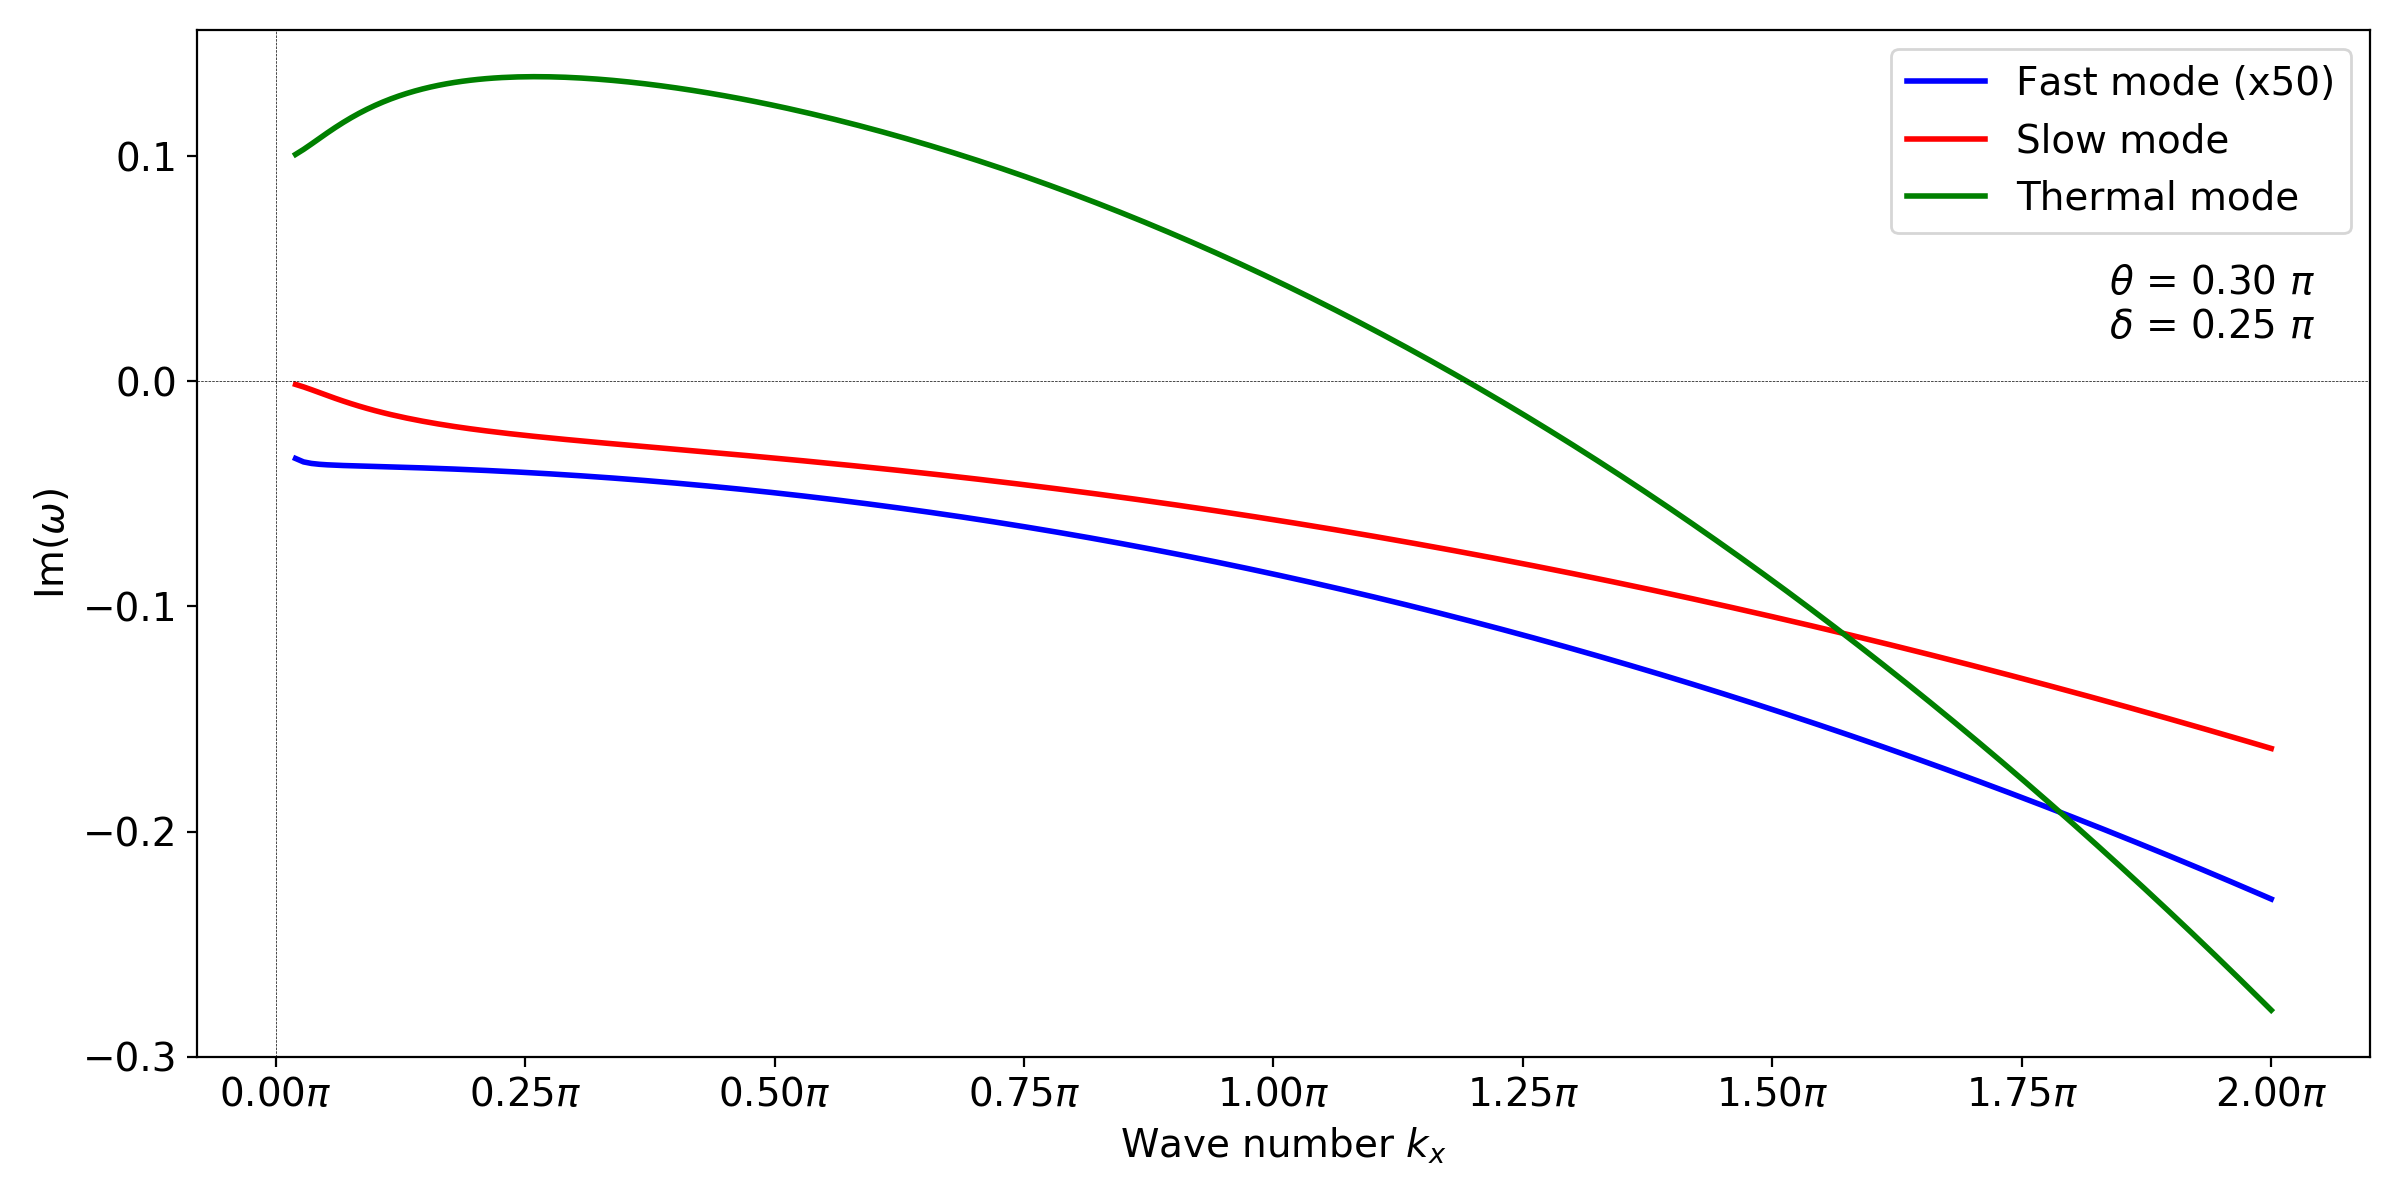
\includegraphics[width=\textwidth]{w_vs_kx.png}
  \caption{
    Growth rates of the MHD modes as a function of wave number, for $\bk$ aligned with the $x$-axis for an angle $\theta = 0.3\pi$ and $\delta = \pi/4$. The thermal mode is stable above $k_x \approx 1.2\pi$, which is the critical wave number for these conditions. The growth rate of the fast mode was multiplied by 50 for clarity. The equilibrium temperature is 0.5 MK; the density and magnetic field are the default values.
  }
  \label{fig: w_vs_kx}
\end{figure}

Figure \ref{fig: w_vs_kx} shows the growth rate of all three relevant modes under typical solar coronal conditions, where we now fix the temperature to 0.5 MK and a given field orientation; the growth rates are shown as a function of wave number. The wave vector $\bk$ was taken along the $x$-axis. The slow and fast wave modes are damped everywhere under these conditions, but the thermal mode shifts from stability to instability when going below the critical wave number. The angles $\theta$ and $\delta$ were given a value of $0.3\pi$ and $\pi/4$, respectively. Note that all growth rates are specified in normalised units, with a unit time equal to $t_n \approx 85.87$ seconds.

\begin{figure}[t]
  \centering
  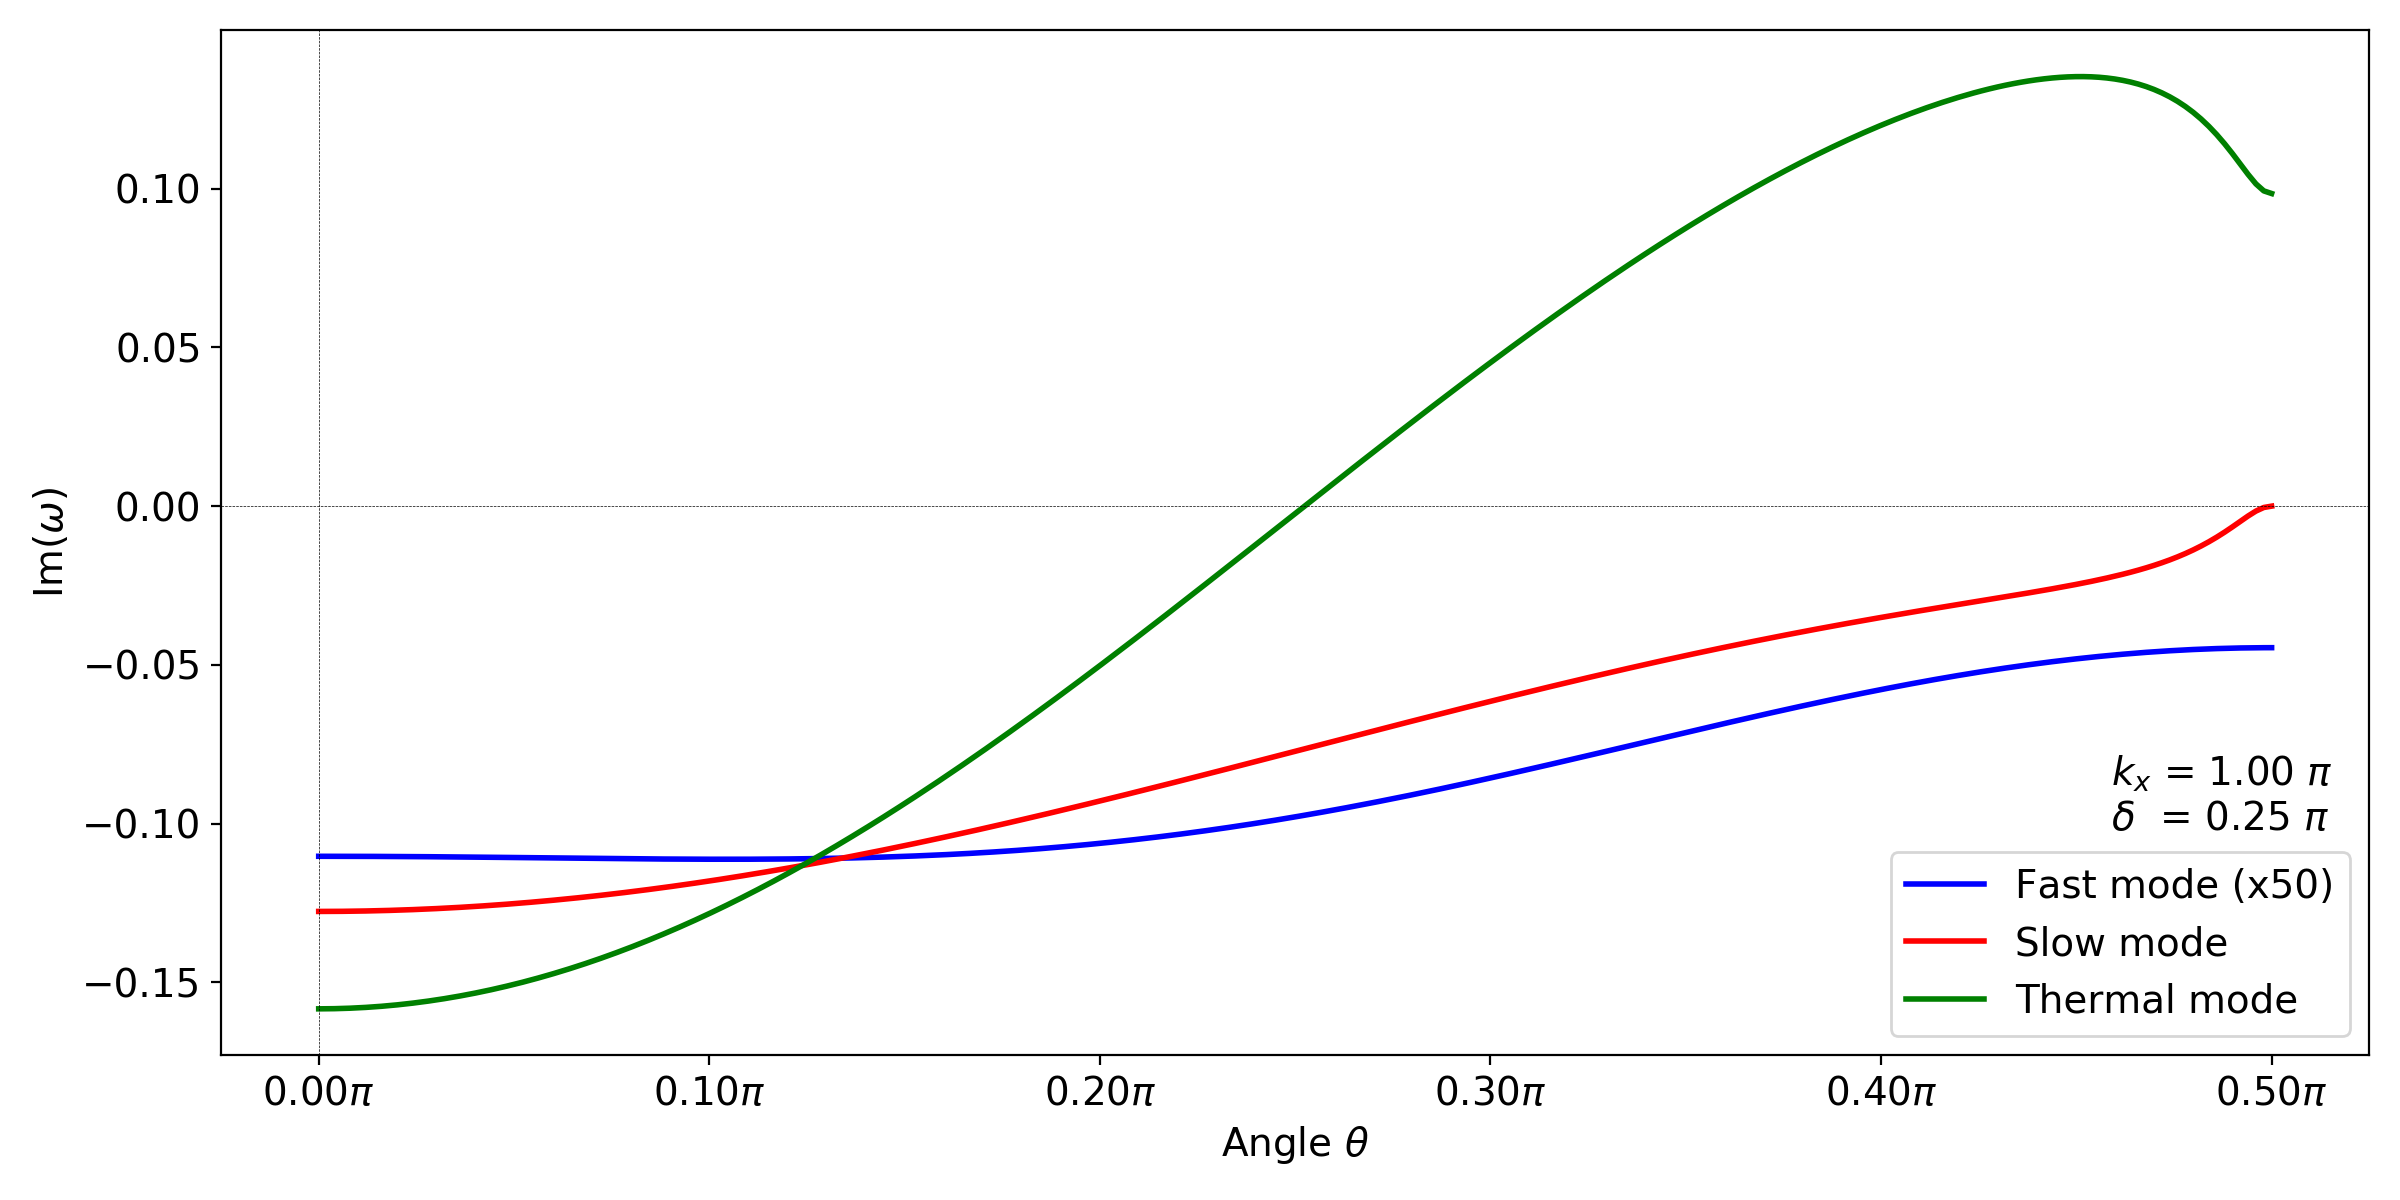
\includegraphics[width=\textwidth]{w_vs_theta.png}
  \caption{
    Growth rates of the MHD modes as a function of $\theta$ for a fixed value of $\delta = \pi/4$ and $k_x = \pi$. The wave vector $\bk$ is aligned with the $x$-axis. The thermal mode becomes unstable for $\theta > \pi/4$, at this point parallel thermal conduction is too ineffective for stabilisation to occur due to the alignment between $\bb_0$ and $\bk$. The growth rate of the fast mode was multiplied by 50 for clarity. The equilibrium temperature is 0.5 MK; the density and magnetic field are the default values.
  }
  \label{fig: w_vs_theta}
\end{figure}

Figure \ref{fig: w_vs_theta} on the other hand indicates that solely considering the critical wave number is not sufficient for instability of the thermal mode. The wave number was taken to be $k_x = \pi$, which according to Figure \ref{fig: w_vs_kx} should indicate instability. However, when the angle $\theta$ is varied and becomes too small (for a fixed $\delta = \pi/4$) the magnetic field becomes too aligned with the wave vector such that the contribution of parallel thermal conduction is particularly effective in smoothing out emerging temperature variations. Only for values of $\theta > \pi/4$ thermal conduction parallel to the field lines becomes inefficient enough, and consequently enables the thermal mode to become unstable under these conditions. Armed with this knowledge, all simulations we perform further on achieve conditions where the slow modes are damped, but the thermal mode is inherently unstable.









\subsection{Synthetic views}
\subsection{Thermal instability onset in 2D}
\subsection{Thermal instability onset in 3D}

\section{Implications and the road ahead}
\cleardoublepage
